\documentclass[11pt]{article}

\usepackage[margin=1.7cm]{geometry}
\usepackage{amsmath}
\usepackage{amssymb}
\usepackage{enumitem}
\usepackage{titlesec}
\usepackage{xcolor}
\usepackage{fancyhdr}
\usepackage{tikz}
\usetikzlibrary{arrows.meta,positioning}

\titleformat{\section}{\large\bfseries}{\thesection}{0.6em}{}
\titlespacing{\section}{0pt}{1.1em}{0.5em}

\pagestyle{fancy}
\fancyhf{}
\fancyhead[L]{Probability Trees and Relative Risk}
\fancyhead[R]{Name: \makebox[4cm]{\hrulefill}}
\fancyfoot[C]{\thepage}
\renewcommand{\headrulewidth}{0.4pt}

\newcommand{\ans}{\hrulefill}
\setlist[enumerate,1]{leftmargin=1.4em, itemsep=0.5em, topsep=0.2em}
\setlist[enumerate,2]{leftmargin=1.3em, itemsep=0.3em, topsep=0.2em}

% \anshere -- a full-width answer line on its own, for questions needing more than a short inline blank
\newcommand{\anshere}{\par\vspace{0.3em}\noindent\ans\par\vspace{0.3em}}

% \drawbox{height} -- a bordered blank space for students to draw their own tree
\newcommand{\drawbox}[1]{%
  \par\noindent\fbox{%
    \begin{minipage}[t][#1][t]{\dimexpr\linewidth-2\fboxsep-2\fboxrule}
      \vspace{0.2em}\hspace{0.2em}\textit{\small Draw your tree here.}
    \end{minipage}%
  }\par%
}

\begin{document}

\begin{center}
  {\Large\bfseries Probability Trees and Relative Risk}
\end{center}

\vspace{0.3em}
\noindent A \textbf{probability tree} shows every possible outcome of two or more events, one stage at a time.
\begin{itemize}[leftmargin=1.4em, itemsep=0.1em, topsep=0.2em]
  \item Label every branch with its probability. The branches leaving any single point must add up to $1$.
  \item To find the probability of a path (a sequence of outcomes), \textbf{multiply} the probabilities along the branches.
  \item To find the probability of several different paths (e.g.\ ``at least one''), \textbf{add} the probabilities of those paths.
\end{itemize}

\vspace{0.5em}
\section*{Worked Example}
\noindent A fair coin is flipped twice. Here is the completed probability tree.

\begin{center}
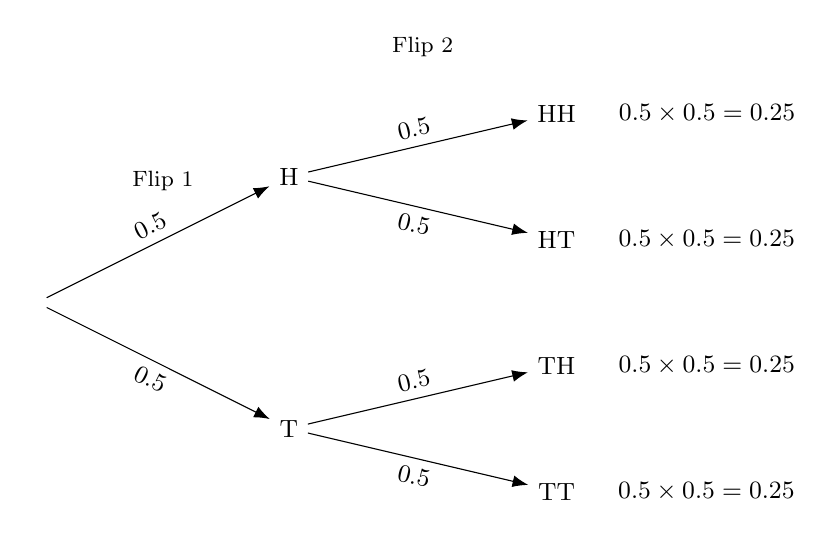
\begin{tikzpicture}[
  level1/.style={font=\small},
  every node/.style={font=\small}
]
\node (S) at (0,0) {};
\node (H1) at (3.2,1.6) {H};
\node (T1) at (3.2,-1.6) {T};
\node (HH) at (6.6,2.4) {HH};
\node (HT) at (6.6,0.8) {HT};
\node (TH) at (6.6,-0.8) {TH};
\node (TT) at (6.6,-2.4) {TT};

\draw[-{Latex[length=2mm]}] (S) -- (H1) node[midway, above, sloped] {$0.5$};
\draw[-{Latex[length=2mm]}] (S) -- (T1) node[midway, below, sloped] {$0.5$};

\draw[-{Latex[length=2mm]}] (H1) -- (HH) node[midway, above, sloped] {$0.5$};
\draw[-{Latex[length=2mm]}] (H1) -- (HT) node[midway, below, sloped] {$0.5$};
\draw[-{Latex[length=2mm]}] (T1) -- (TH) node[midway, above, sloped] {$0.5$};
\draw[-{Latex[length=2mm]}] (T1) -- (TT) node[midway, below, sloped] {$0.5$};

\node[right=0.3cm of HH] {$0.5 \times 0.5 = 0.25$};
\node[right=0.3cm of HT] {$0.5 \times 0.5 = 0.25$};
\node[right=0.3cm of TH] {$0.5 \times 0.5 = 0.25$};
\node[right=0.3cm of TT] {$0.5 \times 0.5 = 0.25$};

\node[above] at (1.6,1.3) {\footnotesize Flip 1};
\node[above] at (4.9,3.0) {\footnotesize Flip 2};
\end{tikzpicture}
\end{center}

\noindent Check: the four outcome probabilities add up to $0.25+0.25+0.25+0.25 = 1$. \quad
$P(\text{at least one head}) = 1 - P(TT) = 1 - 0.25 = 0.75$.

\newpage
\section{Draw Your Own Probability Trees}
\noindent For each scenario: draw and label a complete probability tree (including the outcomes and their probabilities at the end of each path), then answer the question(s).

\begin{enumerate}

\item A spinner is divided into 3 equal sections: Red, Blue and Green. It is spun twice.
\drawbox{5.2cm}

\noindent Find $P(\text{both spins are the same colour})$. \ans

\item A bag contains 4 red marbles and 1 blue marble. A marble is drawn, its colour is noted, and it is \textbf{put back} in the bag. A second marble is then drawn.
\drawbox{5.2cm}

\noindent Find $P(\text{at least one blue marble is drawn})$. \ans

\newpage
\item The same bag (4 red, 1 blue) is used again, but this time the first marble is \textbf{not} put back before the second marble is drawn.
\drawbox{5.2cm}

\begin{enumerate}
  \item Find $P(\text{both marbles are red})$. \ans
  \item Explain why $P(\text{both marbles are blue})$ must be $0$.\anshere
\end{enumerate}

\newpage
\item The probability that it rains on Monday is $0.4$. If it rains on Monday, the probability it also rains on Tuesday is $0.7$. If it does \textbf{not} rain on Monday, the probability it rains on Tuesday is $0.3$.
\drawbox{5.2cm}

\begin{enumerate}
  \item Find $P(\text{it rains on both days})$. \ans
  \item Find $P(\text{it rains on exactly one of the two days})$. \ans
\end{enumerate}

\item A box contains 10 electronic components, 3 of which are defective. Two components are selected at random, one after the other, \textbf{without replacement}, for testing.
\drawbox{5.2cm}

\begin{enumerate}
  \item Find $P(\text{both components are defective})$. \ans
  \item Find $P(\text{at least one component is defective})$. \ans
\end{enumerate}

\newpage
\item In a certain population, $2\%$ of people have a particular disease. A screening test correctly identifies $90\%$ of people who \textbf{have} the disease as positive, and correctly identifies $95\%$ of people who do \textbf{not} have the disease as negative.
\drawbox{5.6cm}

\begin{enumerate}
  \item Find $P(\text{a randomly chosen person has the disease \emph{and} tests positive})$. \ans
  \item Find $P(\text{a randomly chosen person tests positive})$, using both branches that lead to a positive result.\anshere
\end{enumerate}

\end{enumerate}

\newpage
\section{Relative Risk}
\noindent \textbf{Relative risk} compares how likely an event is in one group compared to another group.
\[
  \text{Relative risk (RR)} = \dfrac{\text{risk in Group A}}{\text{risk in Group B}}, \qquad \text{where risk} = \dfrac{\text{number with the outcome}}{\text{total number in the group}}.
\]
If $RR = 1$, the risk is the same in both groups. If $RR > 1$, Group A has a higher risk. If $RR < 1$, Group A has a lower risk.

\begin{enumerate}
  \item In a drug trial, 400 people took a new medicine and 20 of them experienced side effects. 600 people took a placebo (an inactive dummy pill) and 18 of them experienced side effects.
  \begin{enumerate}
    \item Find the risk of side effects for the medicine group. \ans
    \item Find the risk of side effects for the placebo group. \ans
    \item Calculate the relative risk of side effects for the medicine group compared to the placebo group. \ans
    \item Write a sentence interpreting your answer to part (c).\anshere
  \end{enumerate}

  \item Out of 250 smokers studied, 45 developed a certain lung condition. Out of 750 non-smokers studied, 30 developed the same condition.
  \begin{enumerate}
    \item Find the risk of developing the condition for smokers. \ans
    \item Find the risk of developing the condition for non-smokers. \ans
    \item Calculate the relative risk of developing the condition for smokers compared to non-smokers. \ans
    \item Write a sentence interpreting your answer to part (c).\anshere
  \end{enumerate}

  \item Look back at your probability tree for Question 6 in Section 1 (the disease screening test).
  \begin{enumerate}
    \item What is the risk (probability) of testing positive for someone who \textbf{has} the disease? \ans
    \item What is the risk (probability) of testing positive for someone who does \textbf{not} have the disease? \ans
    \item Calculate the relative risk of testing positive for someone with the disease, compared to someone without the disease.\anshere
  \end{enumerate}
\end{enumerate}

\end{document}
